The architecture of the network that allows the existence of Bitcoin is of type \textit{Peer-to-Peer} (P2P).\\This means that each node participating in the network is equal to the others and collaborates with the others by providing the services and functionalities defined by the shared protocol, which is executed by all nodes in a similar manner. Being the antithesis of the most well-known and widely used architecture in the current context, defined as \textit{Client/Server} (C/S), the Bitcoin network does not require centralized servers to provide any type of service. On the contrary, each node constitutes a point in the network, attributing decentralization and resilience to the protocol that only \textit{Peer-to-Peer} networks can guarantee. Examples of P2P networks that have been very successful are those used for file-sharing, initially popularized by \textit{Napster} in 1999, and later evolved into better protocols, such as \textit{BitTorrent}.\\

\noindent Similarly to the aforementioned implementations, Bitcoin was designed to be a \textit{Peer-to-Peer} system for the management and use of digital money, capable of functioning without the intervention of central authorities, with the specific goal of being an uncensorable and resilient tool against centralized control, distributed among the nodes that want to participate in the network. Due to these characteristics, the chosen design for Bitcoin could only be a P2P network.

\subsection{Bitcoin network nodes: types and roles}
The functionalities that nodes can perform to be part of the network are those defined by the Bitcoin protocol, and they can be identified in Figure \ref{fig:nodo}.
Based on the functionalities that each node decides to implement, several categories of nodes can be outlined:
\begin{itemize}
\item Full Node
\item Simplified Payment Verification Node (SPV)
\item Miner Node
\end{itemize}

A \textit{full node} is a node that is responsible for maintaining a complete copy of the Bitcoin blockchain, keeping it up to date through constant communication with other nodes in the network. By having a local copy, it can verify every new transaction or block that arrives without depending on third-party nodes. At the time of writing, the technical requirements to implement a full node remain quite accessible, both in terms of hardware (2GB of RAM, 500GB of free disk space) and technical know-how, thanks to the abundance of online guides and "plug-and-play" style implementations (Figure \ref{fig:umbrel}) developed over the years. It is worth emphasizing the importance, for true decentralization, of having the lowest possible technological barrier: the higher the number of full nodes, the more distributed the network is, resulting in increased overall robustness and resilience. 
\begin{wrapfigure}{r}{0.5\textwidth}
\centering
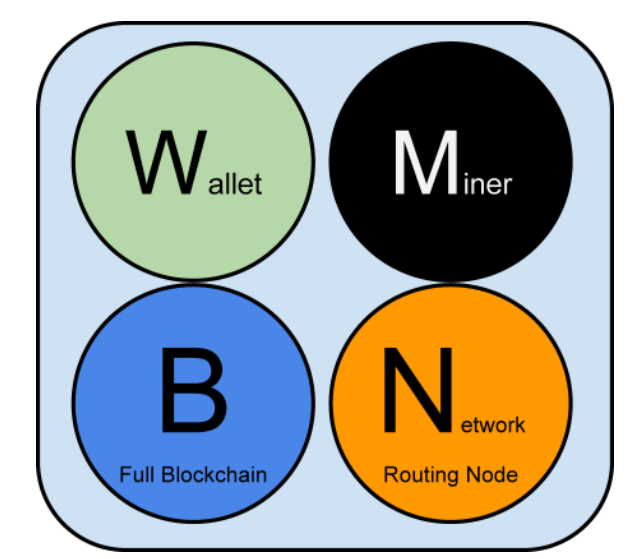
\includegraphics[width=0.45\textwidth]{Figures/bitcoin/tipo1.png}
\caption{Functionalities that a node participating in the Bitcoin network can have.}
\label{fig:nodo}
\end{wrapfigure}
A \textit{Simplified Payment Verification (SPV) node}, on the other hand, contains a copy of all block headers but not the transactions and other data related to them. It verifies the validity of the headers of new blocks and is also able to verify transactions of interest with the help of a connected full node. For this reason, nodes of this type are also called lightweight nodes. The main advantage of this category of nodes is their lower use of hardware resources (disk space) compared to full nodes, making them more suitable for contexts with stricter resource limitations (e.g., smartphones). The main disadvantage of SPV nodes is their dependence on other full nodes when they require a specific series of blocks that they do not have locally. During this process, a \textit{Sybil attack} could occur, compromising the privacy of an SPV client. To overcome and mitigate this risk, \textit{bloom filters} have been introduced. \cite{bitcoinopsTransactionBloom}
A \textit{Miner node}, unlike the previous types, has the specific purpose of solving the \textit{Proof-of-Work (POW)} algorithm in order to claim the reward for a new block. It uses increasingly specialized hardware, such as Application Specific Integrated Circuits (ASICs), which have been the norm for several years now (see Figure \ref{fig:asic}). Once a miner solves the block they are working on, they communicate the solution to the rest of the network through their full node or by transmitting the new block to a connected node. At that point, transactions contained in that mined block are considered confirmed, since they are included in a block and subsequent blocks will be added on top, forming a chain of confirmations. The number of confirmations increases the level of trust in the transactions.

\begin{figure}[!ht]
    \begin{minipage}[t]{0.52\textwidth}
    \centering
    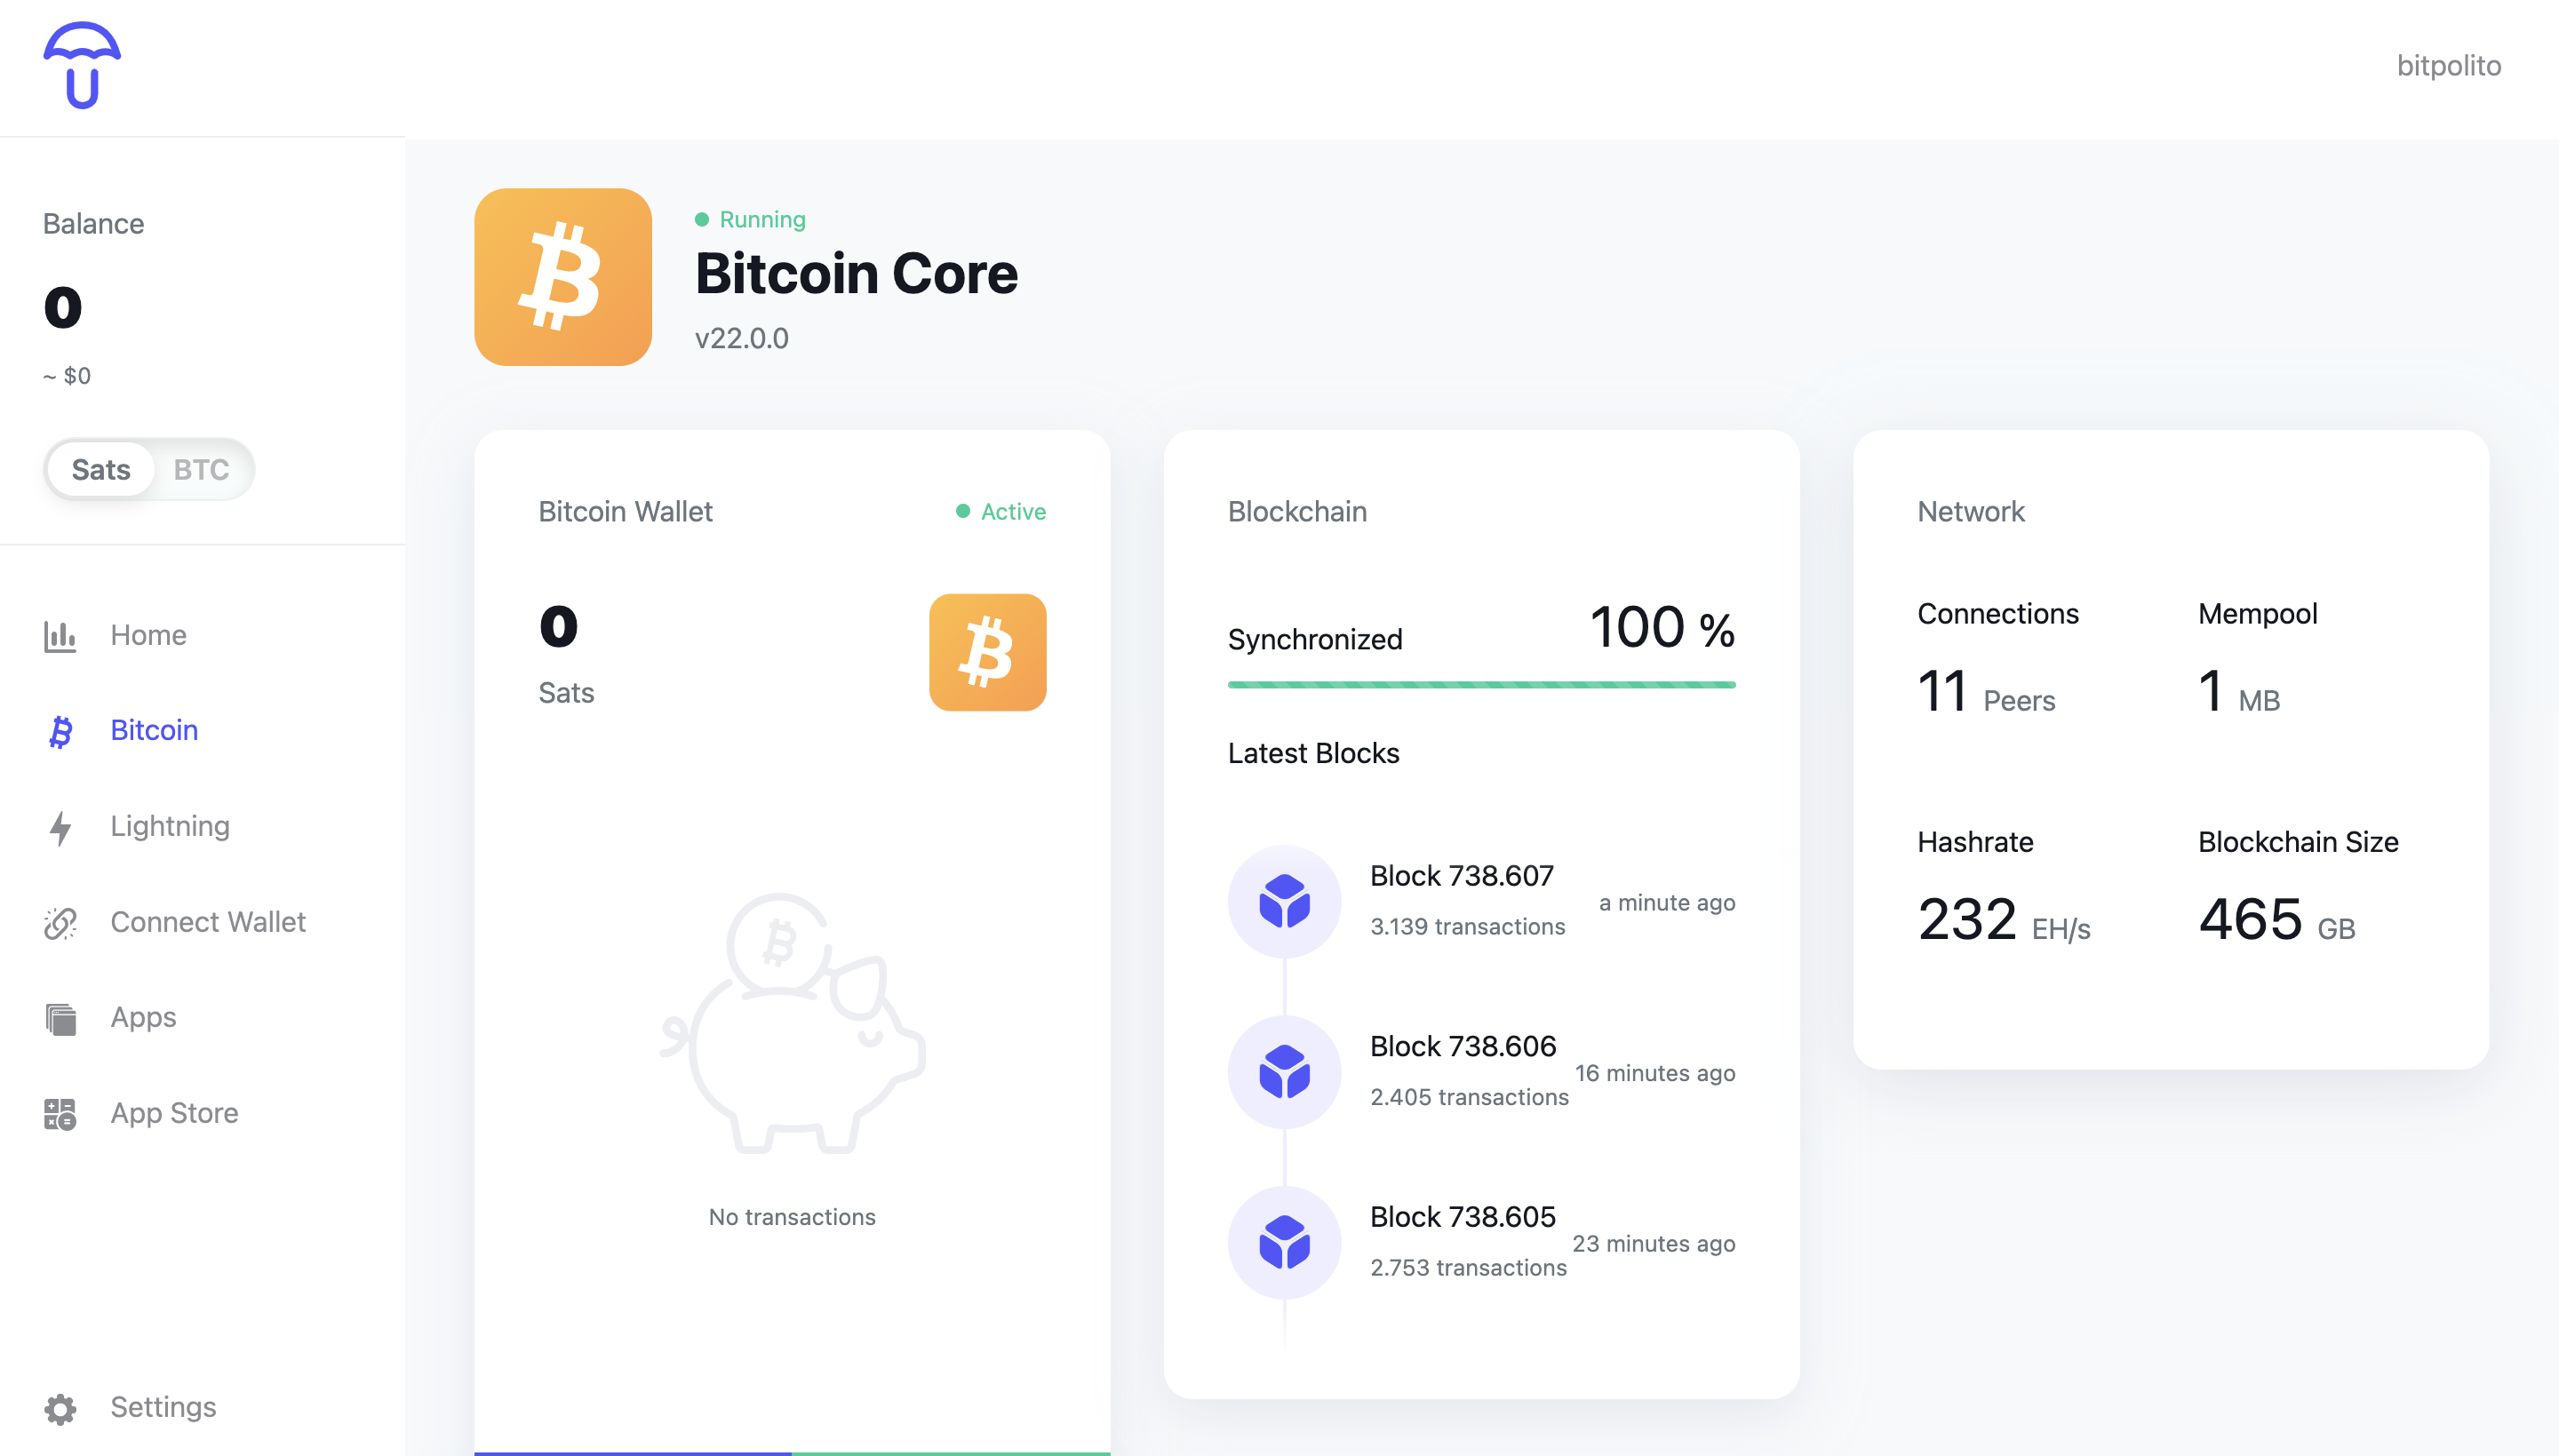
\includegraphics[width=1.1\textwidth]{Figures/bitcoin/bitpolito-node.png}
    \caption{Umbrel implementation of a Bitcoin full node}
    \label{fig:umbrel}
    \end{minipage}\hfill
    \begin{minipage}[t]{0.35\textwidth}
    \centering
    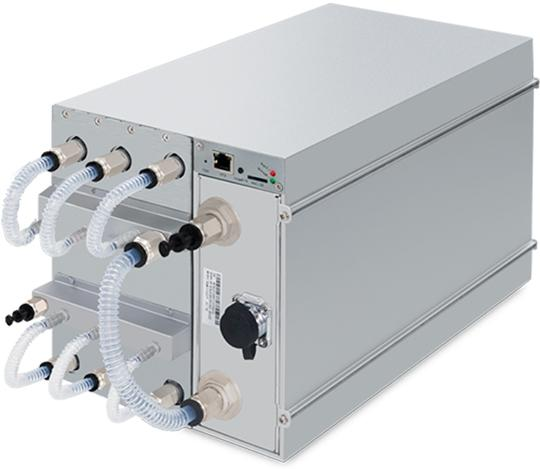
\includegraphics[width=1\textwidth]{Figures/bitcoin/s19xp.jpg}
    \caption{Antminer S19XP Hydro, one of the most powerful ASIC machines for Bitcoin mining}
    \label{fig:asic}
    \end{minipage}
\end{figure}


\subsection{Extended Bitcoin network}

The composition of the network described above represents the basic functioning of the Bitcoin P2P protocol. Actually, Bitcoin network is further enriched by other nodes that execute specific protocols (e.g. Stratum, FIBRE). An overview of the so-called \textit{Extended Bitcoin Network} can be better understood through Figure \ref{fig:extended_network}.
Analyzing the map, three protocols (highlighted in different colors) can be observed, which are fully compatible with each other and allow various interactions between different types of nodes, depending on the functionalities each node decides to implement and make available to the extended network.
For example, a portion of the network is strongly connected to a \textit{Pool Server}, which consists of a series of nodes responsible for mining operations by aggregating their hash power in a mining pool. This is done to reduce the inherent variance associated with Proof-of-Work. The pool server manages communication and interaction through its own protocol specifically developed for these mining operations. The opposite of pooled mining is represented by nodes called \textit{Solo Miners}. They do not rely on any mining pool for their mining operations and require a local copy of the blockchain (indicated by the blue dot within the nodes) to independently verify new transactions before starting the search for the \textit{nonce}. All the differences between Solo Mining and Pooled Mining will be deeply discussed and analyzed in Chapter \ref{chapt:mining}. 
The protocol represented by the red connections is called the \textit{Stratum Protocol}. It was developed around 2012 as an alternative to the previous pooled mining model. The goal of Stratum is to define a kind of standard for managing communications between mining pool servers and miners. This pooled mining protocol will be deeply discussed and analyzed in section \ref{section:stratum}.
\begin{figure}[h!]
\centering
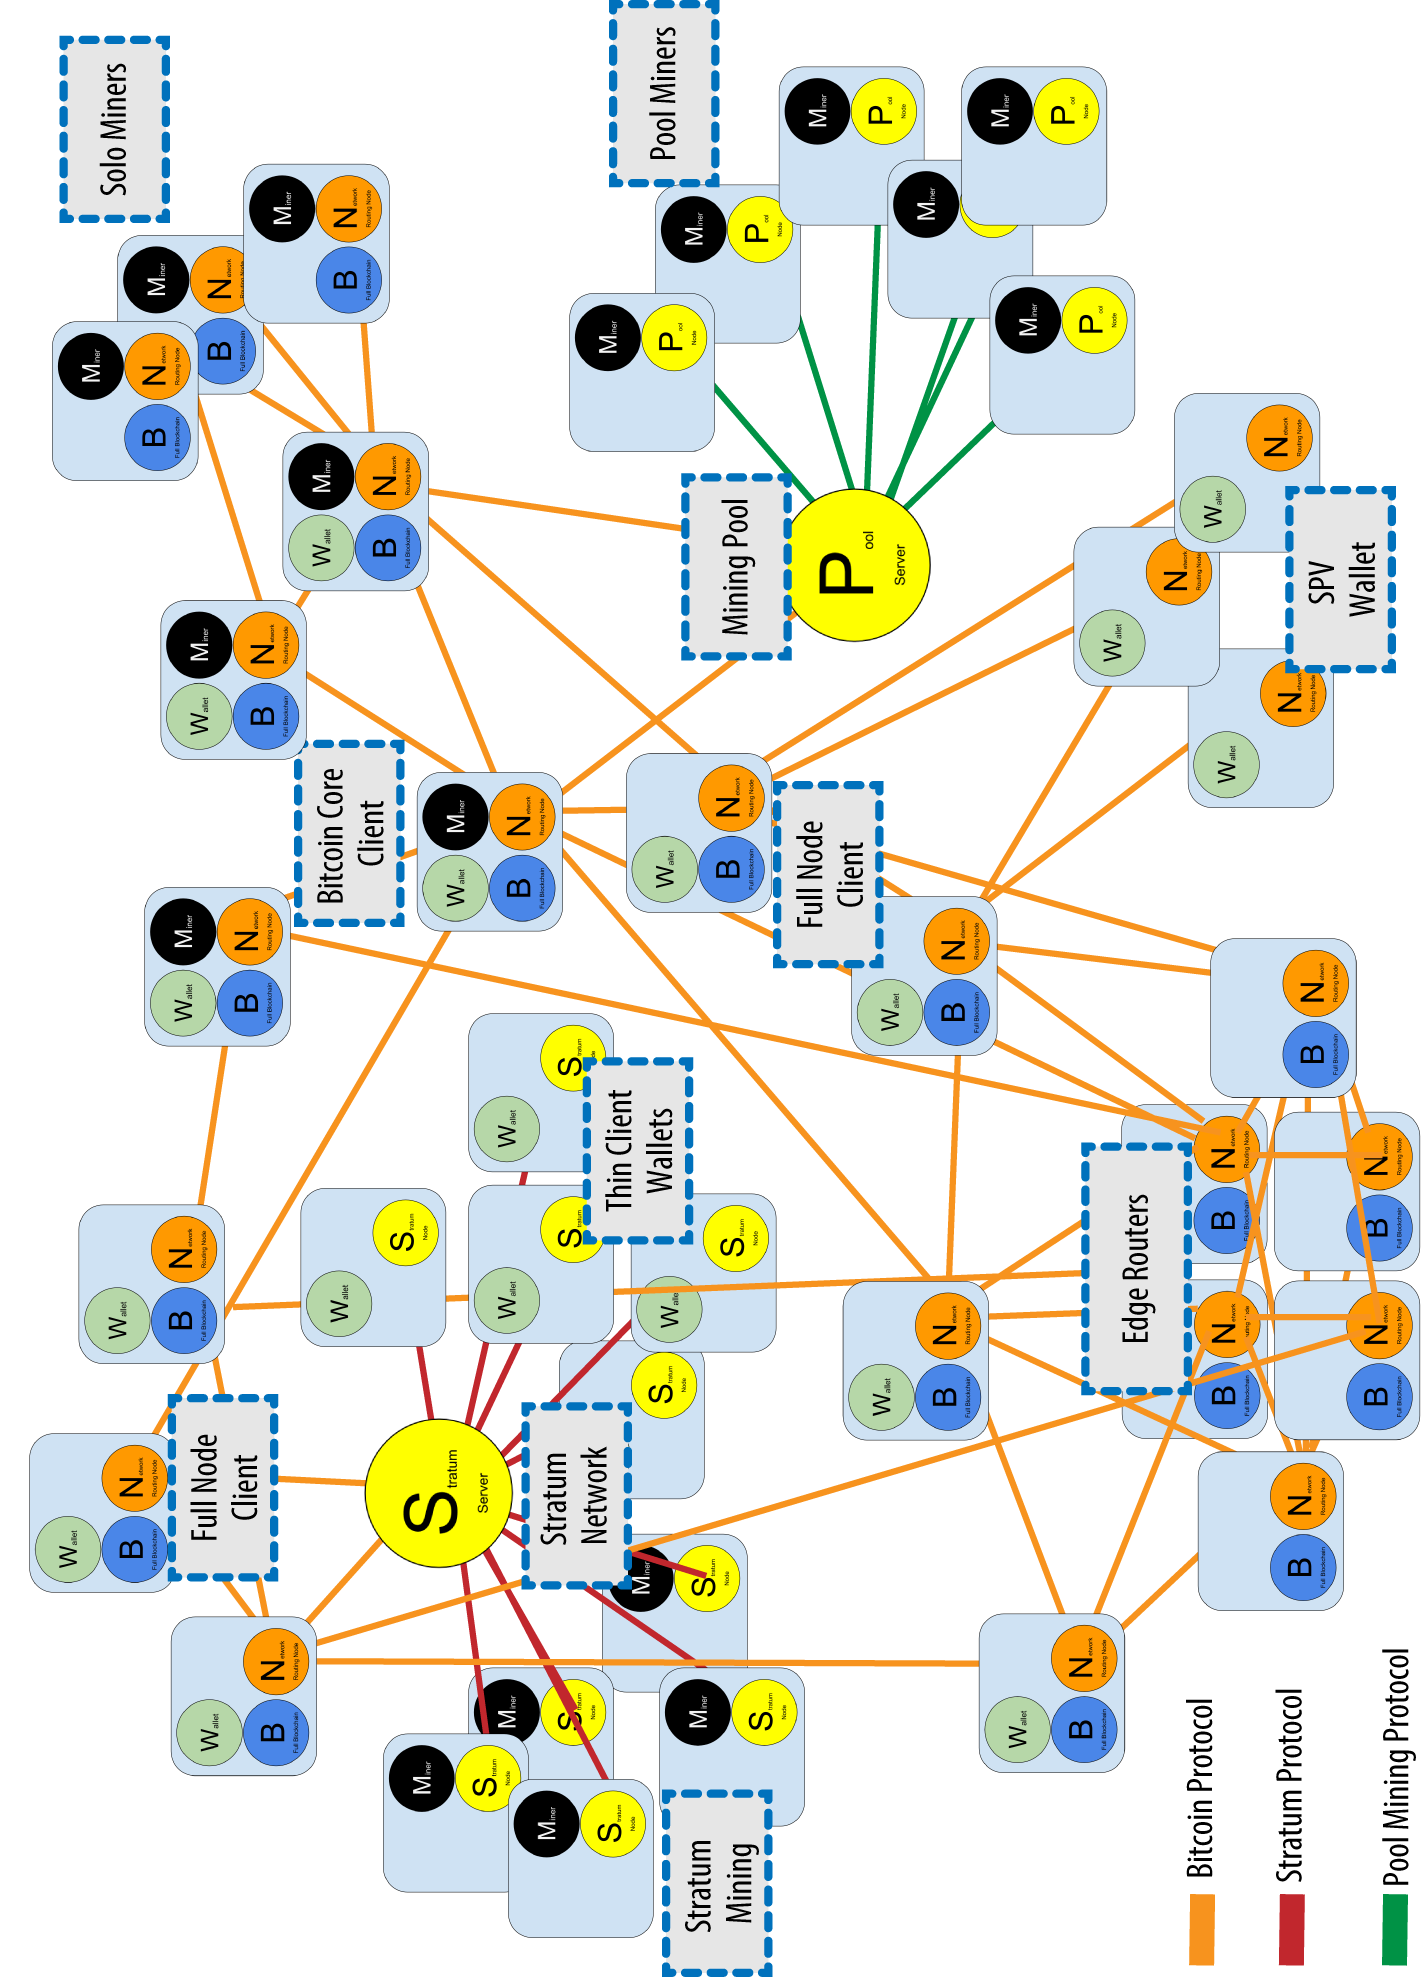
\includegraphics[width=11cm,angle=270,origin=c]{Figures/bitcoin/tipo3.png}
\caption{Map of the "Extended Bitcoin Network."}
\label{fig:extended_network}
\end{figure}

\subsection{Geographical distribution and statistics}

Using certain functions defined within the Bitcoin protocol, implemented and made available by most nodes, it is possible to perform a recursive search of the connections present between nodes and obtain some statistics related to the global geographical distribution of the Bitcoin network. It is important to note that many popular implementations for creating a personal full node in a more user-friendly way (such as Umbrel, RaspiBlitz, MyNode, or RoninDojo) operate through the Tor network. In these cases, the IP address detected by Bitnodes does not geolocate the actual physical location of the node but rather the Tor exit node to which it is connected. \\
Based on the data collected from Bitnodes.io, at the time of writing, the entire Bitcoin network consists of approximately 17,000 reachable nodes. The term "reachable" refers to nodes that accept new incoming connections, providing access to new nodes and allowing them to download the entire blockchain starting from the genesis block. On the same website, it is possible to find the estimate of the total number of nodes (both reachable and unreachable), which currently exceeds 44,000 nodes. \cite{bitnodesGlobalBitcoin}

\noindent In addition to statistics on countries and cities worldwide, another interesting data point is the percentage of nodes that are updated to the latest version of the Bitcoin protocol (25.0.0), which is approximately 23\%. Regarding the data on Autonomous System Numbers (ASNs) identified by Bitnodes.io's crawlers, it can be observed that around 60\% of nodes communicate through the Tor network, while only 2.3\% are hosted on AWS servers.

\begin{figure}[h!]
\centering
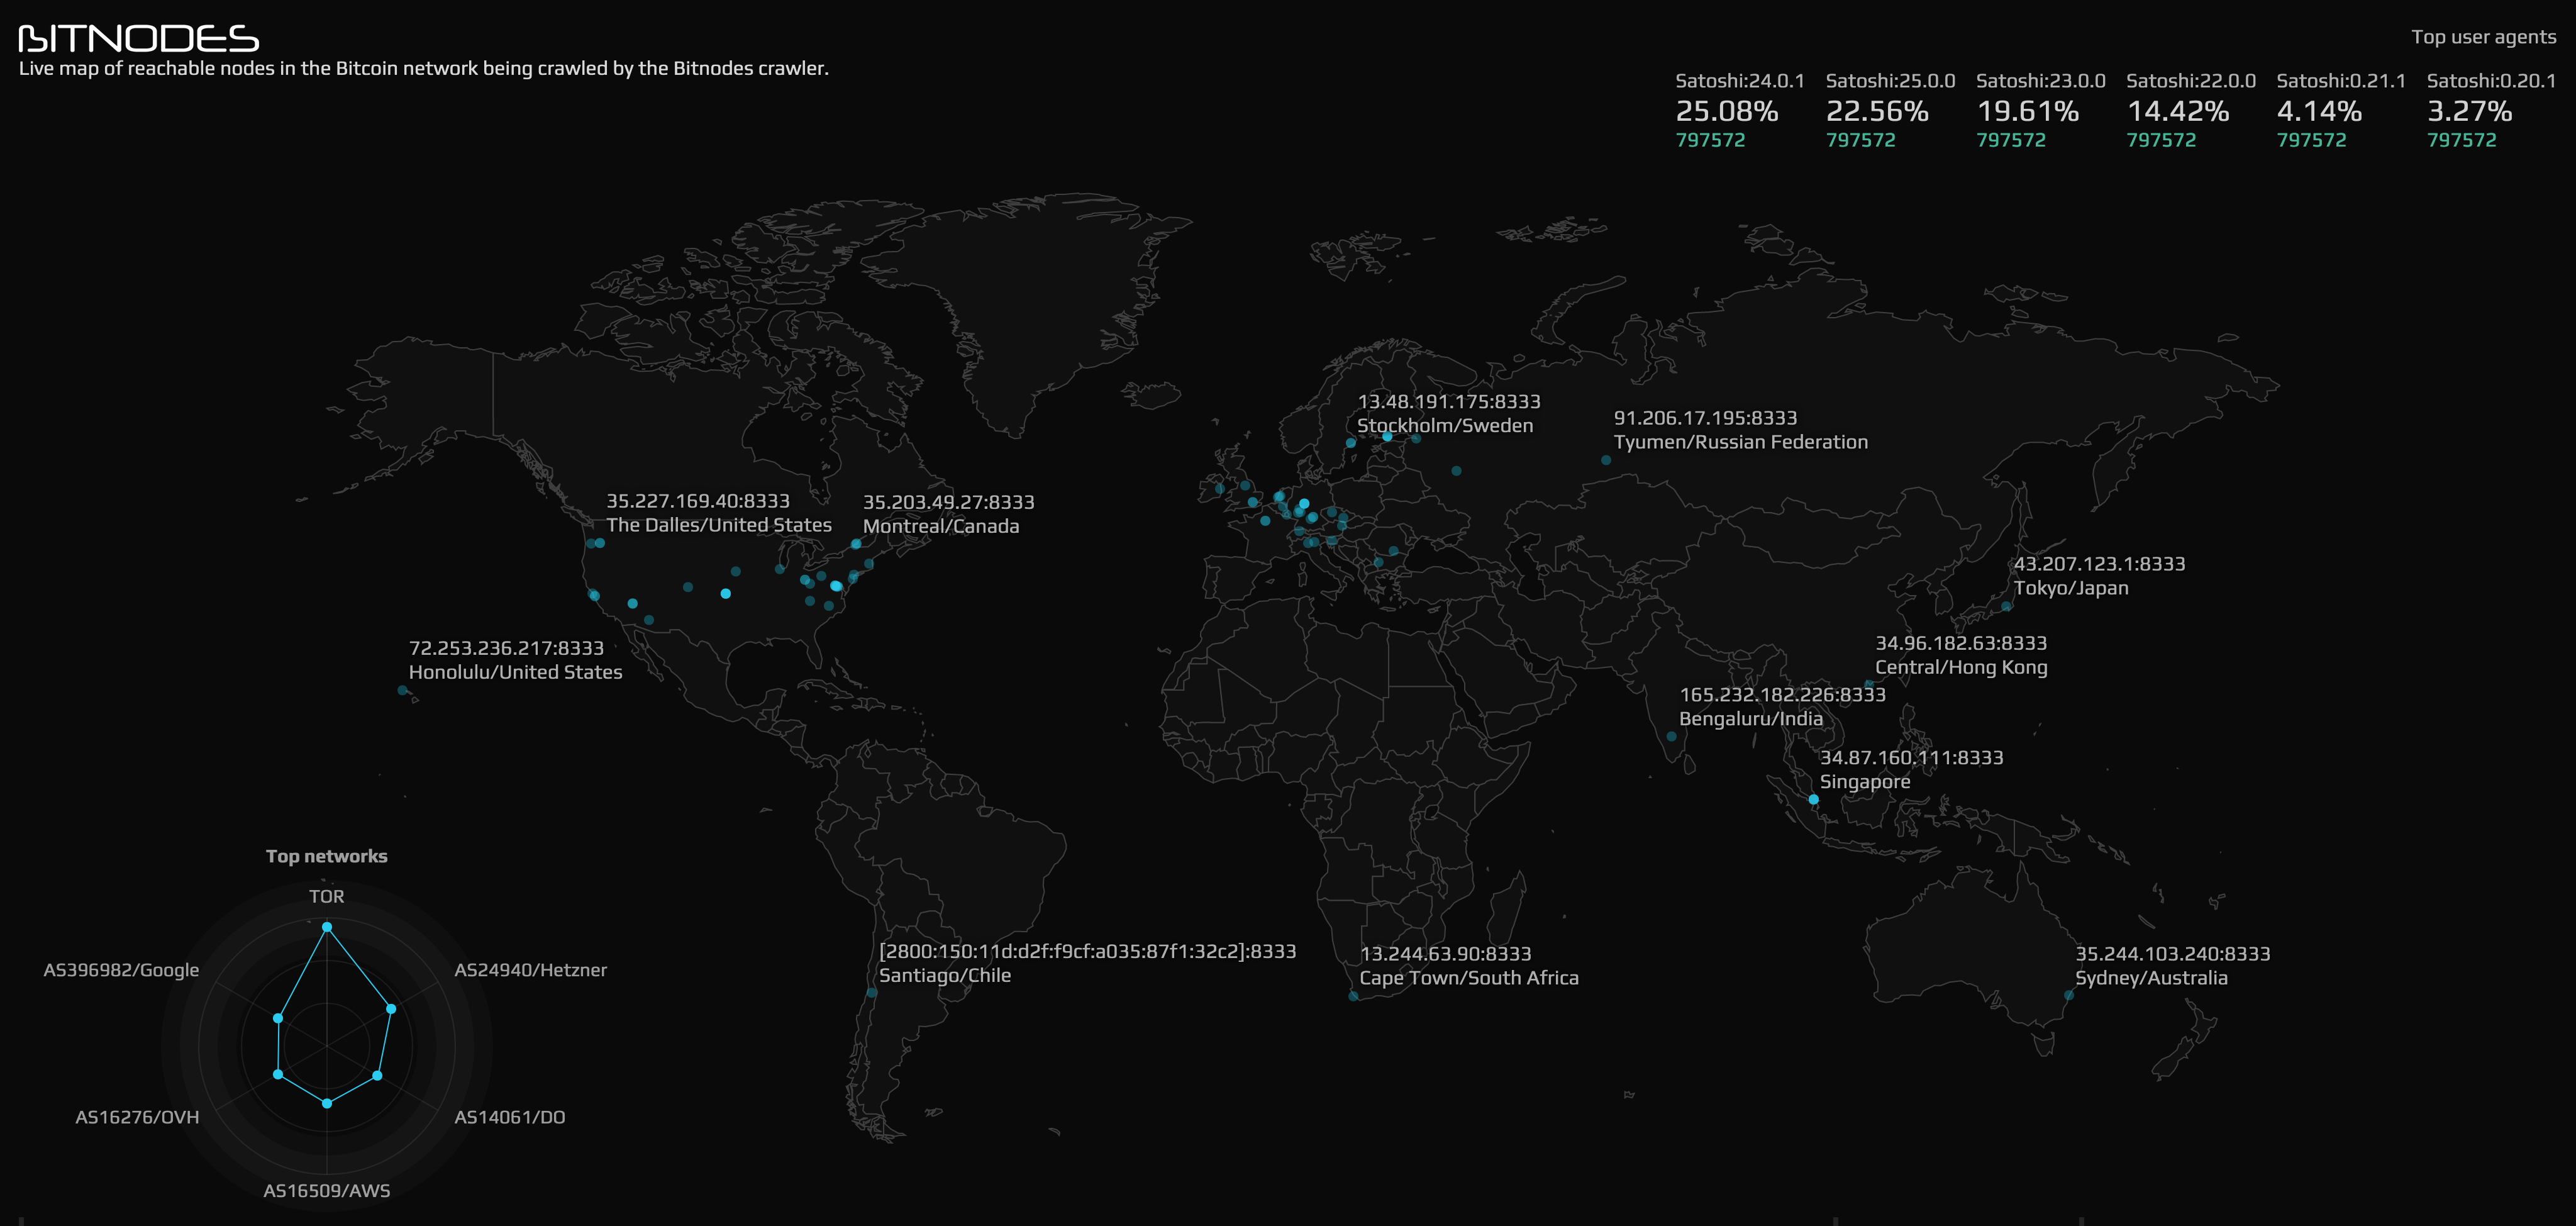
\includegraphics[width=15cm]{Figures/bitcoin/bitmap1.png}
\caption{Screenshot of the live map on Bitnodes.io.}
\label{fig:live_map}
\end{figure}